\section{Limited Area Modelling}

This section follows up on a discussion initiated by Prof. Myoshi in Vienna \cite{Raynaud2024}. Upon conducting research, I came across a publication by Joel Oskarsson et al. \cite{LAM}. To deepen my understanding of this domain, I should read this \href{https://www.researchgate.net/publication/349484799}{chapter}.\\

The title of the article is "Graph-based Neural Weather Prediction for Limited Area Modeling." In this article, the authors present an implementation of a neural weather prediction system based on graph theory. The article describes three models: GC-LAM, 1L-LAM, and HI-LAM.\\

The first two models, GC-LAM and 1L-LAM, are direct implementations of the GraphCast model. In GraphCast, the boundaries of each node's domain have different resolutions, enabling the propagation of long-range physical phenomena while maintaining precision for local phenomena.\\

HI-LAM introduces an innovation by proposing different node architectures adapted to various resolutions. This approach addresses the problem of nodes having less information than others. In HI-LAM, all nodes receive the same information, eliminating certain artifacts along the edges of the nodes.\\

\begin{figure}[ht]
\centering
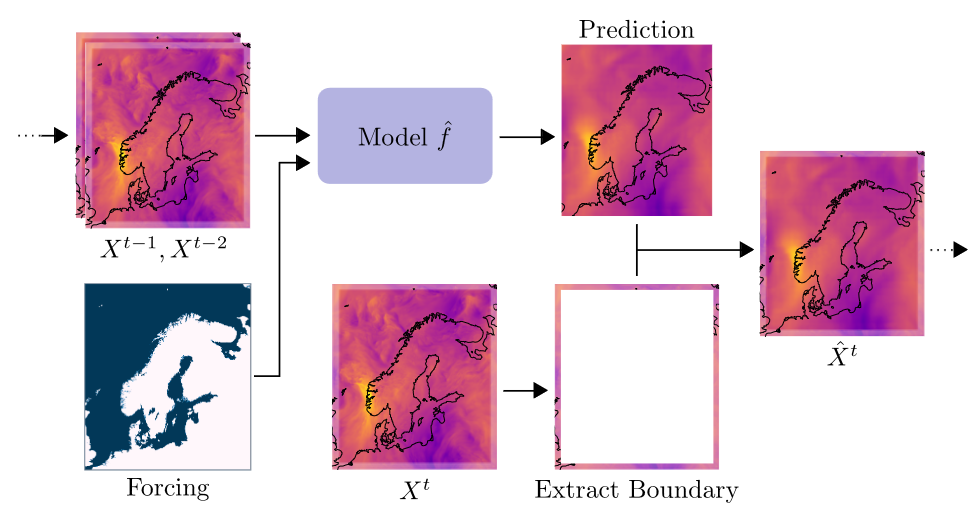
\includegraphics[width=0.9\textwidth]{media/LAM_Boundary-Forcing.png}
\caption{Boundary forcing in the case of a LAM}
\label{fig}
\end{figure}

A specific consideration is how the boundary conditions are obtained. To address this issue, before each iteration, an expanded domain is given to the algorithm to define the forcing (see figure \ref{fig}). One question that arises is whether this expanded domain is sufficient, or if a global model should be provided to the system for more relevant predictions. Furthermore, in an operational context, we would be required to use a global model to extract this information at each time step. Therefore, a low-resolution global model coupled with a high-resolution local model would be advantageous.